\chapter{Background\label{cha:chapter2}}
This chapter addresses the theoretical and contextual background 
necessary to understand the key concepts and methodologies 
that form the foundation of the current research.
The first section will discuss the basics of deep neural networks (NNs), 
upon which the technical setup of this thesis is based.
The next section aims to provide a broader context for the term \textit{quantization}, 
followed by a final section that explains the common NN modification techniques 
used in learned quantization scenarios.

\section{Fundamentals of Deep Learning}
\label{sec:section2}
This section introduces the fundamental concepts of deep learning, 
beginning with the most basic NN architecture and progressing to loss functions with regularization. 
The concepts of the forward pass and backpropagation will be explained in the last subsection.

\subsection{Dense Layers in Neural Networks}
\label{subsec:subsection1}
NNs can be considered a mathematical abstraction of the human decision-making process. 
Consider a scenario where, given an image, you need to say aloud what you see. 
The two eyes can be regarded as input nodes that receive the initial data, 
the brain can be seen as the hidden layer that processes this data, 
and your mouth — the output node that provides the final answer.
\\
\\
The hidden layer, which typically consists of many neurons, is where the magic
 — or the transformation of data — happens. In its simplest form, 
 within the classic \textit{Multilayer Perceptron} (MLP) model,
 each hidden layer neuron performs a weighted operation:

\[
\textit{output} = f(w \cdot \textit{input} + b)
\]
\\
\noindent where:

\begin{itemize}
  \item \textit{input} refers to the outputs from the previous layer (or the initial data from input nodes in our case) that are fed into a specific neuron in the hidden layer.
  \item \textit{w} (weights) is a vector of parameters associated with that specific neuron, defining the importance of each input received by this neuron. 
  \item \textit{b} (bias) is an additional scalar parameter specific to the neuron, which shifts the result of the weighted sum, allowing for more flexibility.
  \item \textit{f} is the \textit{activation function}, a nonlinear function applied to the weighted sum of inputs and bias in that specific neuron, allowing for more complexity.
  \item \textit{output} is the result produced by the neuron, which will then be passed on to the next hidden layer or to the final output layer.
\end{itemize}

\noindent Hidden layers where each neuron is connected to every neuron in the previous layer 
and every neuron in the next layer are called \textit{dense layers}.


\begin{figure}[h!]
  \centering
  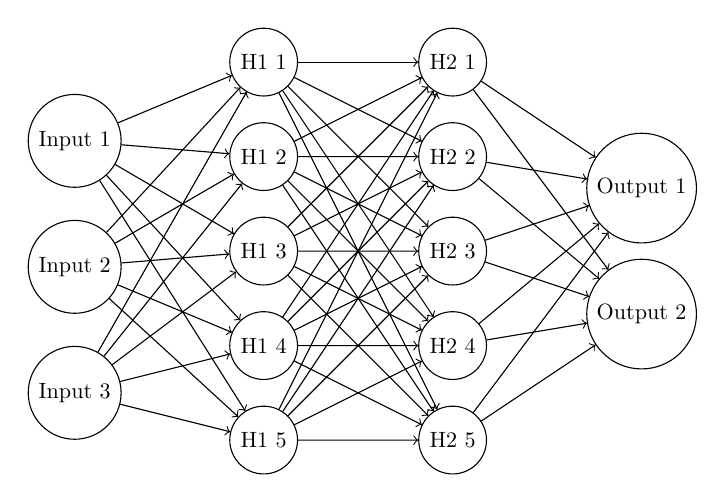
\begin{tikzpicture}[scale=0.8, every node/.style={transform shape}]

      % Input Layer
      \foreach \i in {1,...,3}
        \node[draw, circle, minimum size=0.8cm] (I-\i) at (0,-2.0*\i) {Input \i};
      
      % Hidden Layer 1
      \foreach \i in {1,...,5}
        \node[draw, circle, minimum size=0.8cm] (H1-\i) at (3,-1.5*\i+0.75) {H1 \i};
      
      % Hidden Layer 2
      \foreach \i in {1,...,5}
        \node[draw, circle, minimum size=0.8cm] (H2-\i) at (6,-1.5*\i+0.75) {H2 \i};
      
      % Output Layer
      \foreach \i in {1,...,2}
        \node[draw, circle, minimum size=0.8cm] (O-\i) at (9,-2.0*\i-0.75) {Output \i};
      
      % Connecting layers
      \foreach \i in {1,...,3}
        \foreach \j in {1,...,5}
          \draw[->] (I-\i) -- (H1-\j);
      
      \foreach \i in {1,...,5}
        \foreach \j in {1,...,5}
          \draw[->] (H1-\i) -- (H2-\j);
      
      \foreach \i in {1,...,5}
        \foreach \j in {1,...,2}
          \draw[->] (H2-\i) -- (O-\j);
      
  \end{tikzpicture}
  \caption{Multilayer Perceptron with Two Dense Hidden Layers}
  \label{fig:mlp_diagram}
\end{figure}


\noindent This interconnectedness of dense layers introduces the inherent redundancy of NNs. 
It is particularly true in models with a large number of neurons, where the \textit{weight matrix}
\( W \) — made up of the weight vectors \( w \) for each neuron in the layer — results 
in a vast number of parameters, many of which have little influence on the final output.
Thus, customizing these dense layers will be one of the key focus points in the current work.


\subsection{Loss Functions \& Regularization}
\label{subsec:subsection2}
The weights and biases are usually \textit{learnable parameters}
that the model adjusts during \textit{training}.
The training process of NNs is similar to how our brains learn from mistakes. 
Given the ground truth, a NN adjusts its learnable parameters 
using a specific function that compares the ground truth with the output generated by the network, 
essentially measuring the magnitude of the network's errors.
\\
\\
This function is called a \textit{loss function}, and depending on the type of question the network aims to answer, it can take many different forms.
For example, for the MLP described in Figure~\ref{fig:mlp_diagram} that generates a binary classification, we would use the \textit{log loss} function. 
Since the datasets used in this thesis involve multi-class classification, the \textit{sparse categorical cross-entropy} (SCCE) loss function will be used, 
which measures the difference between the predicted class probabilities and the true labels for each class in the dataset.
\\
\\
Often the loss function alone is not enough for a NN to perform well. This is why a \textit{regularization term} that penalizes unwanted behaviours
is added to the loss function.
\\
\\
A typical regularization term is \( L_2 \), 
which penalizes large weights by adding the sum of the squared weights to the loss function. 
The modified loss function is expressed as:

\[
\mathcal{L}_{\text{total}} = \mathcal{L}_{\text{data}} + \lambda \sum_{i} w_i^2
\]
\\
\noindent where:

\begin{itemize}
  \item \( \mathcal{L}_{\text{data}} \) is the original loss function (in our case, the SCCE loss function).
  \item \( \lambda \) is a scalar parameter that controls the strength of the regularization.
  \item \( w_i \) represents each individual weight value in the model.
\end{itemize}

\noindent The current work employs multiple custom regularization terms 
that encourage specific behaviors in the models while discouraging others. 
These terms will be discussed in detail in the Experimental Setup section.
\\
\\
THIS PART WILL GO TO THE NEXT SECTION:
\\
\\
An example approach is to define a regularization term that directly penalizes large differences between full-precision values 
and their quantized counterparts \cite{zhuang2018towards}. This can encourage the model to learn parameters that are easily quantizable without significant performance loss.
If the values that are being quantized are \( W \), then this regularization term could look like:

\[
\mathcal{L}_{\text{quant}} = \lambda \sum_{i} \| W_i - q(W_i) \|^2
\]

\noindent Where:
\begin{itemize}
    \item \( \lambda \) is a scalar that controls the importance of the quantization penalty.
    \item \( W_i \) represents the full-precision weight value before quantization at index \( i \).
    \item \( q(W_i) \) represents the quantized version of \( W_i \).
\end{itemize}

\noindent The current work uses multiple custom regularization terms that trigger the quantization process during training. 
These will be discussed in detail in the Experimental Setup section.

\subsection{Forward-Pass \& Back-Propagation}
\label{subsec:subsection2}
The repetition of the operation described earlier in the Dense Layers in Neural Networks subsection during model training 
is essentially the forward pass. It is the process where input data is passed through the network layer by layer, 
with each layer applying its learned weights and biases to produce a final output. 
\\
\\
As mentioned in the previous subsection, this output is then compared with the ground truth by the loss function that produces an error.
This error is used to update the learnable parameters — in case of MLPs, the values in \( W \) and \( b \) — during a process called back-propagation.
\\
\\
In other words, back-propagation is the method by which the network adjusts its parameters to minimize the error. 
It calculates the gradient of the loss function with respect to each parameter using the chain rule. 
\( W \) and \( b \) are typically updated as follows:

\[
W = W - \eta \frac{\partial L}{\partial W}, \quad b = b - \eta \frac{\partial L}{\partial b}
\]
\\
\noindent where \( L \) is the loss function, and \( \eta \) is the learning rate.
\\
\\
For example, consider the weight \( W_{I1,H1_1} \) represented as the line between \textit{Input 1} and the hidden layer node \( H1_1 \) in Figure~\ref{fig:mlp_diagram}. 
The gradient of this weight with respect to the loss is calculated using the chain rule:

\[
\frac{\partial L}{\partial W_{I1,H1_1}} = \frac{\partial L}{\partial \text{Output 1}} \cdot \frac{\partial \text{Output 1}}{\partial H1_1} \cdot \frac{\partial H1_1}{\partial W_{I1,H1_1}}
\]

\noindent Where:
\begin{itemize}
    \item \( \frac{\partial L}{\partial \text{Output 1}} \) is the gradient of the loss with respect to \textit{Output 1}.
    \item \( \frac{\partial \text{Output 1}}{\partial H1_1} \) is the gradient of \textit{Output 1} with respect to the output of \( H1_1 \).
    \item \( \frac{\partial H1_1}{\partial W_{I1,H11}} \) is the value of \textit{Input 1}, since \( H1_1 \) is a weighted sum of the inputs.
\end{itemize}

\noindent This shows how each weight contributes to the final error during back-propagation.

\section{Quantization}
\label{sec:section1}
This section aims to answer the \textit{why} question with respect to quantization and further provides a broader understanding of the term regarding its types.

\subsection{Purpose \& Definition}
\label{subsec:subsection1}
With humans becoming increasingly dependent on deep learning models disguised as everyday tools — such as facial recognition filters, 
document scanners, self-driving cars, and more — the need for these models to function in a resource- and 
time-efficient manner is more imperative than ever. Among the many ways to meet this need, 
quantization has become one of the most common techniques used to reduce the computational 
and memory costs of deep NNs, given the sheer amount of parameters they possess and the inherent redundancy this introduces.
\\
\\
While the term \textit{quantization} has its roots in the first half of the 20th century \cite{gray1998quantization}, in the context of NNs, 
it has gained renewed importance  — the over-parameterization of NNs introduces a certain type of flexibility 
that allows quantization to be implemented in many different forms \cite{gholami2021survey}.
Despite the abundance of these forms and approaches, quantization of NNs generally refers to the process of 
reducing the bit precision of their parameters, all while maintaining accuracy within an acceptable range.

\subsection{Quantization Types}
\label{subsec:subsection2}

Although there is a multitude of ways to classify NN quantization methods, the most general classification is the division between \textit{static, dynamic}, and \textit{learned quantization}.
    \begin{itemize}
        \item In \textbf{static quantization}, quantization parameters are fixed before model inference, based on the data observed during training or calibration.
        This corresponds to Post-Training Quantization (PTQ), which directly quantizes the trained floating-point model \cite{jiang2021efficient}, 
        using various discretization approaches based on the range and distribution of the parameters being quantized, 
        as well as the level of granularity at which the quantization values are applied.
        
        \item In \textbf{dynamic quantization}, the quantization parameters are calculated dynamically during inference. 
        This typically applies to activations, as their range changes depending on the input data and, unlike that of the weights, 
        cannot be precomputed with static quantization \cite{kim2021ibert}.
        
        \item In \textbf{learned quantization}, quantization parameters are learned as part of the model training process.
        This corresponds to Quantization Aware Training (QAT) \cite{jacob2018quantization}, where quantization is integrated directly into training rather than applied afterwards.
        Since learned quantization is central to this work, a detailed review of QAT and its applications is provided in the Related Work chapter. 

    \end{itemize}

\section{Common Concepts of QAT}
\label{sec:section2}
Now that the fundamentals of deep learning have been covered, 
this section introduces concepts commonly encountered in learned quantization, 
including the modified forward-pass technique and the challenges it creates for back-propagation.
\subsection{Low-Precision Forward-Pass}
\label{subsec:subsection1}
In QAT, the operation performed during the forward-pass is often modified. Instead of propagating the full precision values, 
the output of a layer is first quantized and then dequantized before being passed to the next layer \cite{jacob2018quantization}. 
This simulates the effect of quantization during inference, helping the network adjust to the reduced precision parameters.
\\
\\
The \textit{quantization} process can be generalized as follows:

\[
q(x) = \text{round}\left( \frac{x}{P} \right) - Z
\]
\\
\noindent where \( q(x) \) is the quantized value, \( x \) is the full precision value of the parameter that is being quantized, \( P \) is a quantization parameter, such as a scaling factor, 
and \( Z \) represents the zero point. This method is the most commonly used \textit{uniform quantization}, which can be either \textit{asymmetric} or \textit{symmetric}, 
depending on the value of \( Z \), with  \( Z \) = 0 representing \textit{symmetric quantization}.
\\
\\
For \textit{dequantization}, we apply:

\[
x_{\text{dequant}} = P \cdot ( q(x) + Z)
\]
\\
\noindent Note that the dequantized value does not necessarily match the initial value. 
For example, if \( x = 7.8 \) and \( P = 2 \), then quantization gives \( q(x) = 4 \), and dequantization results in \( x_{\text{dequant}} = 8 \). 
This demonstrates how the \textit{quantization} and dequantization process approximates the original value \( x \)
by rounding it to the nearest representable value based on the quantization parameter \( P \).

\subsection{Full-Precision Back-Propagation}
\label{subsec:subsection1}
In QAT, although the forward-pass operates on quantized values, back-propagation typically uses full-precision values. 
This is because the rounding operation in the forward-pass is non-differentiable, which makes it impossible to compute gradients directly.
\\
\\
Consider the example of computing the gradient of the weight \( W_{I1,H1_1} \) in Figure~\ref{fig:mlp_diagram}:

\[
\frac{\partial L}{\partial W_{I1,H1_1}} = \frac{\partial L}{\partial \text{Output 1}} \cdot \frac{\partial \text{Output 1}}{\partial H1_1} \cdot \frac{\partial H1_1}{\partial W_{I1,H1_1}}
\]
\\
\noindent If the output of \( H1_1 \) was quantized using a rounding operation, the gradient 
\[
\frac{\partial H1_1}{\partial W_{I1,H1_1}} 
\]
would be undefined due to the non-differentiability of rounding. This would break the gradient flow, making it impossible to update  \( W_{I1,H1_1} \)
during back-propagation.
\\
\\
To work around this, techniques such as the Straight-Through Estimator (STE) are commonly used \cite{bengio2013estimating} \cite{fan2021training} \cite{zhuang2018towards}.
The STE approximates the gradient by treating the rounding function as if it were differentiable during the back-propagation.
This approach ensures that the model can simulate low-precision inference during the forward pass,
while still benefiting from the accuracy of full-precision gradient updates during back-propagation.
\\
\\
The Experimental Setup section will explain a slighly different version of the typical STE that was used in the current work.